\chapter{Introduksjon}

\section{Optimaliseringsproblemet}

La \(f: \Omega \to \R\) være en kost-funksjon som vi ønsker å maksimere eller minimere, der \(\Omega \subset \R^d\) er mengden av mulige løsninger.

\begin{definition}{Optimeringsproblemet \((P)\)}{optimization_problem}
  \[
    \min_{x \in \Omega} f(x) \quad \text{eller} \quad \max_{x \in \Omega} f(x).
  \]

\end{definition}

\section*{Typer optimering}

\begin{itemize}
  \item \textbf{Ubundet optimalisering (Fri, Gratis)}: Ingen restriksjoner på \(x\) og \(\Omega = \R^d\).
  \item \textbf{Konveks optimalisering}: Restriksjoner på \(x\) og \(\Omega \subset \R^d\).
  \item \textbf{Bundet optimalisering}: Restriksjoner på \(x\) og \(\Omega \subset \R^d\).
\end{itemize}

\section{Matematiske Definisjoner og Notasjon}

\section{Ytre og indre produkter}
\begin{definition}{Ytre produkt}{outer_product}
  Gitt to vektorer \( \symbf{a} \in \R^m \) og \( \symbf{b} \in \R^n \), er det ytre produktet definert som:
  \[
    \symbf{a} \otimes \symbf{b} = \symbf{a} \symbf{b}^\top =
    \begin{bmatrix}
      a_1b_1 & a_1b_2 & \cdots & a_1b_n \\
      a_2b_1 & a_2b_2 & \cdots & a_2b_n \\
      \vdots & \vdots & \ddots & \vdots \\
      a_mb_1 & a_mb_2 & \cdots & a_mb_n
    \end{bmatrix}
  \]
\end{definition}

\begin{definition}{Indre produkt}{inner_product}
  Gitt to vektorer \( \symbf{a}, \symbf{b} \in \R^n \), er det indre produktet definert som:

  \[
    \symbf{a} \cdot \symbf{b} = \symbf{a}^\top \symbf{b} = \sum_{i=1}^{n} a_i b_i
  \]

\end{definition}



\section{Nivåsett}
Intuitivt er nivåsettet til en funksjon \( f \) i et punkt \( y \) mengden av alle punkter \( x \) som har samme eller lavere verdi enn \( y \) under \( f \).
\begin{definition}{Nivåsett}{level_set}
  \(f: \Omega \to \overline{\R}\) er en funksjon. Vi definerer nivåsettet til \(f\) i punktet \(y \in \R\) som:
  \[
    \mathcal{L}_f(y) = \{x \in \Omega | f(x) = y\}.
  \]
\end{definition}

\section{Åpen og lukket mengde}

\begin{definition}{Åpen mengde}{open_set}
  En mengde \(A \subset \R^n\) er åpen hvis for alle \(x \in A\) finnes det en \(\varepsilon > 0\) slik at \(B(x, \varepsilon) \subset A\).
  \[
    \forall x \in A, \exists \varepsilon > 0 \text{ s.a. } B(x, \varepsilon) \subset A
  \]
\end{definition}

\begin{definition}{Lukket mengde}{closed_set}
  En mengde \(A \subset \R^n\) er lukket hvis komplementet \(A^c\) er åpent.
  \[
    A \text{ er lukket} \Leftrightarrow A^c \text{ er åpen}
  \]
\end{definition}

\section{Begrenset mengde}
En mengde er begrenset hvis den ikke strekker seg til uendelig langt i noen retning.
Intuitivt kan vi si at en mengde er begrenset hvis den kan plasseres innenfor en kule med endelig radius.

\begin{definition}{Begrenset mengde}{bounded_set}
  En mengde \(A \subset \R^n\) er begrenset hvis det finnes en \(R > 0\) slik at
  \[
    \norm{x} \leq R \quad \forall x \in A
  \]
\end{definition}

\section{Kompakt mengde}
En kompakt mengde er en mengde som er både lukket og begrenset. Dette betyr at den er avgrenset og inneholder alle sine grenseverdier.

\begin{definition}{Kompakt mengde}{compact_set}
  En mengde \(A \subset \R^n\) er kompakt hvis den er lukket og begrenset.
  \[
    A \text{ er kompakt} \Leftrightarrow A \text{ er lukket og begrenset}
  \]
\end{definition}

\section{Nedre semi-kontinuerlige funksjoner (lsc)}

En nedre semikontinuerlig funksjon (\textit{lower semi-continuous function}) er en funksjon som ikke har plutselige "hopp nedover".

Tenk deg at du nærmer deg et punkt \( \symbf{x_0} \) fra alle mulige retninger:
\begin{itemize}
  \item Verdien av funksjonen i \( \symbf{x_0} \) vil ikke være høyere enn verdiene du ser når du kommer nærmere.
  \item Funksjonen kan ha "hopp oppover".
\end{itemize}


\begin{definition}{Nedre semi-kontinuerlig funksjoner}{lsc}
  \(f: \Omega (\subset \R^d) \to \overline{\R}\) være en funksjon. Vi sier at \(f\) er nedre semi-kontinuerlig (lsc) i punktet \(x_0\) hvis for alle \(\varepsilon > 0\) finnes det en \(\delta > 0\) slik at
  \[
    f(x) > f(x_0) - \varepsilon \quad \text{for alle} \quad x \in B(x_0, \delta).
  \]
  \begin{enumerate}
    \item \(f\) er (lsc) i \(x_0\) hvis det for alle \(\alpha \in \R\) er mengden \(\mathcal{L}_f(\alpha) = \{x | f(x) < \alpha \} \text{ er åpen i } \R^d\)
    \item \(f\) er (lsc) i \(x_0 \in X\) hvis og bare hvis: \(\liminf_{x \to x_0} f(x) \geq f(x_0)\).
  \end{enumerate}
\end{definition}
\begin{example}{Eksempel på en nedre semi-kontinuerlig funksjon}{lsc}
  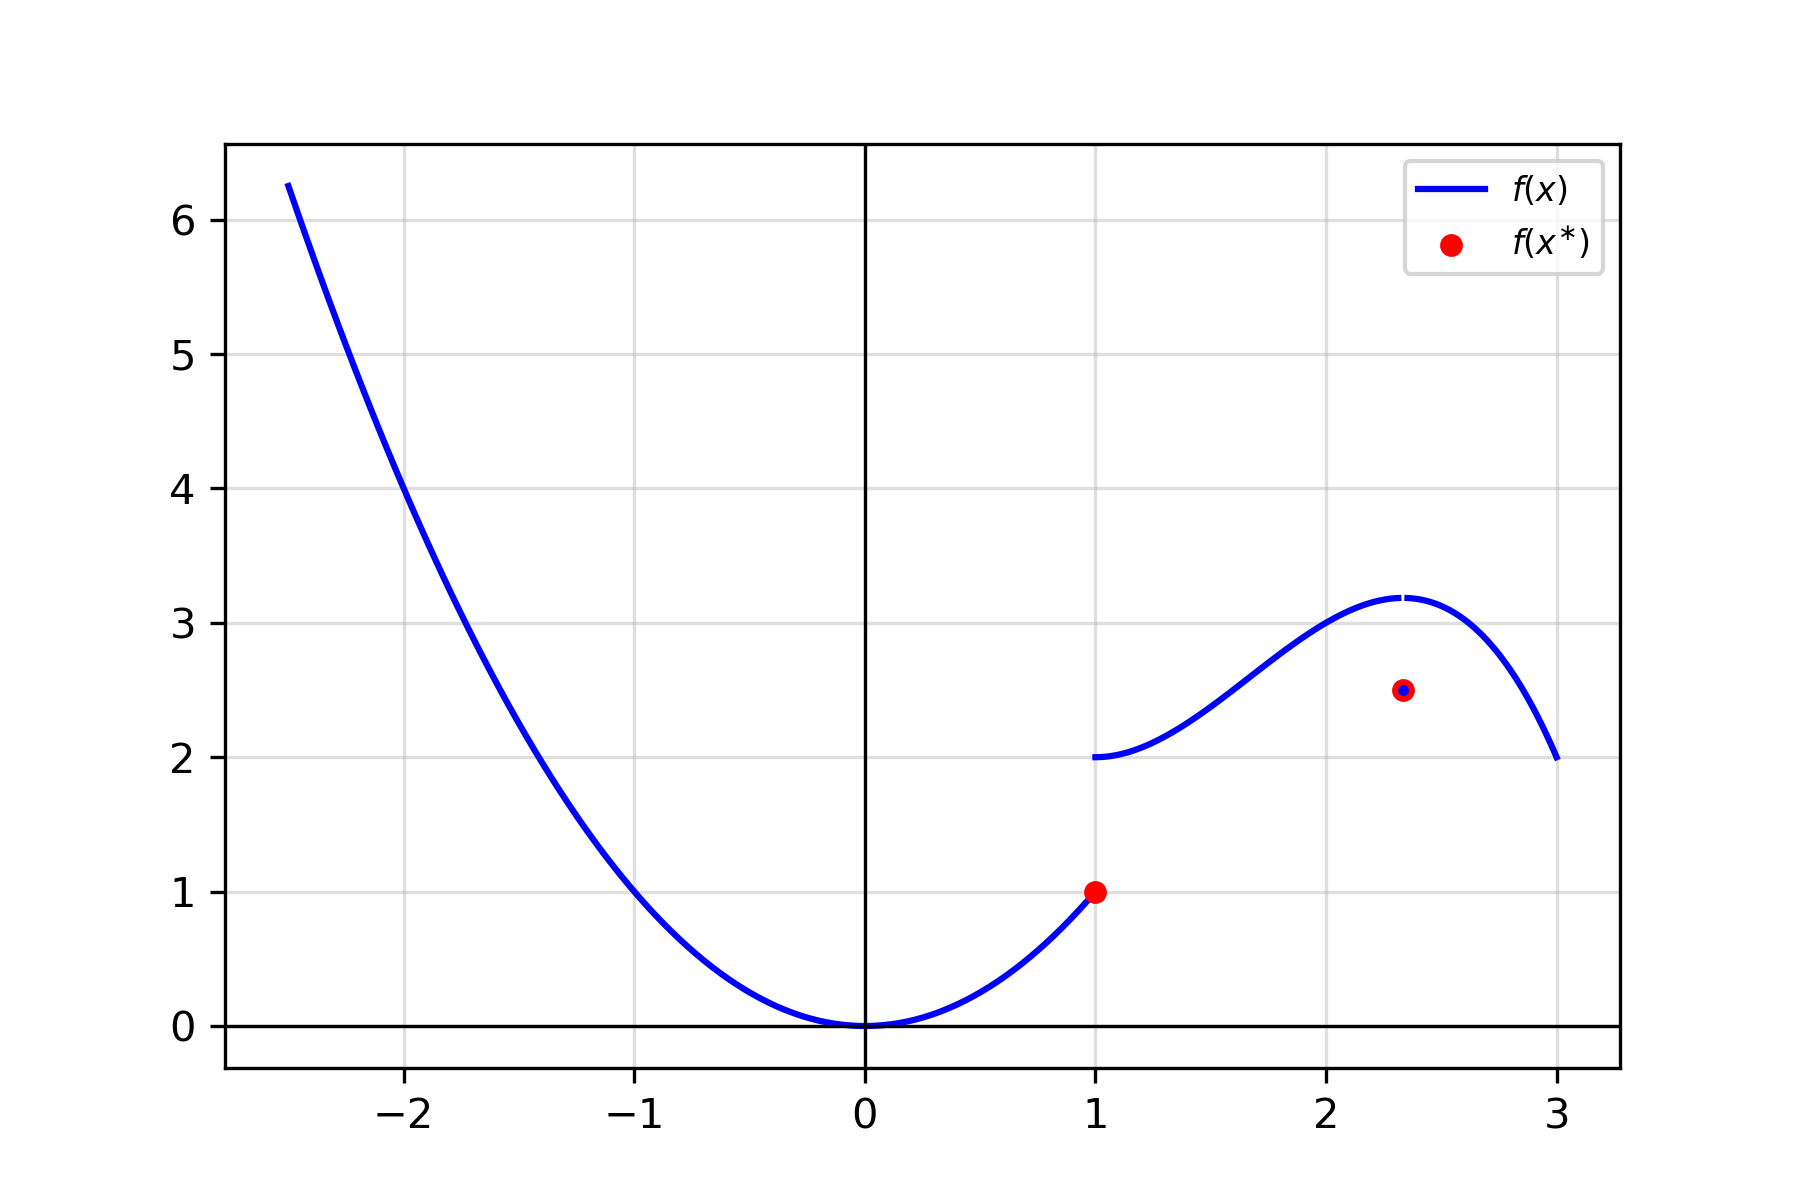
\includegraphics[width=0.5\textwidth]{figures/example_lsc.png}
\end{example}

\section{Koersivitet}

En koersiv funksjon er intuitivt en funksjon som "går mot uendelig" når vi beveger oss mot kanten av definisjonsmengden hvor \( f \) er definert.

\begin{definition}{Koersivitet}{coercive}
  En funksjon \(f: \Omega \to \R\) er koersiv hvis for alle \(y \in \R\) er nivåmengden \(\mathcal{L}_f(y) = \{x \in \Omega | f(x) \leq y\}\) kompakt.

  \[
    \lim_{\norm{x} \to +\infty} f(x) = +\infty
  \]
\end{definition}

\section{Konveksitet}

Konveksitet er en egenskap som beskriver hvordan en funksjon bøyer seg.
En konveks funksjon har en bue som vender oppover, mens en konkav funksjon har en bue som vender nedover.

\begin{definition}{Konveks funksjon}{convex_function}
  En funksjon \(f: \R^n \to \R\) er konveks hvis for alle \(x, y \in \R^n\) og \(\lambda \in [0, 1]\) har vi:

  \begin{align*}
    f(\lambda x + (1 - \lambda)y) & \leq \lambda f(x) + (1 - \lambda)f(y) \\
  \end{align*}

\end{definition}
\begin{remark}{Strengt konveks funksjon}{strictly_convex}
  En funksjon \(f: \R^n \to \R\) er strengt konveks hvis for alle \(x, y \in \R^n\) og \(\lambda \in (0, 1)\) har vi:
  \[
    f(\lambda x + (1 - \lambda)y) < \lambda f(x) + (1 - \lambda)f(y)
  \]
\end{remark}

\begin{remark}{Kvasi-konveks}{quasi_convex}
  En funksjon \(f: \R^d \to \R\) er kvasi-konveks hvis for alle \(x, y \in \R^n\) og \(\lambda \in (0, 1)\) har vi:

  \[
    f(\lambda x + (1 - \lambda)y) \leq \max\{f(x), f(y)\}
  \]

  En alternativ definisjon er at en funksjon er kvasi-konveks hvis alle nivåsettene er konvekse.

  \[
    \mathcal{L}_f(y) = \{x \in \R^n | f(x) \leq y\} \quad \text{er konveks for alle} \quad y \in \R
  \]

  \[
    \boxed{\underbrace{\forall \alpha \in \R, \mathcal{L}_f(\alpha) \text{ er konveks}}_{f \text{ er kvasi-konveks }}\Longleftrightarrow \forall x, y \in \R^d,\lambda \text{ s.a. } f(\lambda x + (1-\lambda)y) \leq \max \{ f(x), f(y) \}}
  \]
\end{remark}


\begin{definition}{Konveks sett}{convex_set}
  En mengde \(C \subset \R^n\) er (strengt) konveks når:

  \begin{align*}
    \lambda x + (1 - \lambda)y & \in C \quad \forall \; x, y \in C, \lambda \in [0, 1] \tag{Konveks}                   \\
    \lambda x + (1 - \lambda)y & \in C \quad \forall \; x, y \in C, \lambda \in (0, 1), x \neq y \tag{Strengt konveks}
  \end{align*}

\end{definition}


\section{Globale og lokale løsninger}

En løsning av et optimeringsproblem er et punkt som oppfyller visse betingelser.
Vi skiller mellom globale og lokale løsninger.

\begin{definition}{Global løsning}{}
  La \(f: \Omega \to \R\) være en funksjon. Vi sier at \(\symbf{x}^* \in \Omega\) er en global løsning av minimeringsproblemet \((P)\) hvis

  \begin{align*}
    f(\symbf{x}^*) & \leq f(\symbf{x}) \quad \text{for alle} \quad \symbf{x} \in \Omega, \tag{Global løsning}                                 \\
    f(\symbf{x}^*) & < f(\symbf{x}) \quad \text{for alle} \quad \symbf{x} \in \Omega, \symbf{x} \neq \symbf{x}^*. \tag{Streng global løsning}
  \end{align*}
\end{definition}

\begin{definition}{Lokal løsning}{}

  La \(f: \Omega \to \R\) være en funksjon. Vi sier at \(x^* \in \Omega\) er en lokal løsning av optimeringsproblemet hvis

  \begin{align*}
    f(\symbf{x}^*) & \leq f(\symbf{x}) \quad \text{for alle} \quad \symbf{x} \in B(\symbf{x}^*, \varepsilon) \cap \Omega, \tag{Lokal løsning}                                     \\
    f(\symbf{x}^*) & < f(\symbf{x}) \quad \text{for alle} \quad \symbf{x} \in B(\symbf{x}^*, \varepsilon) \cap \Omega, \symbf{x} \neq \symbf{x}^*. \tag{Streng lokal løsning}     \\
    f(\symbf{x}^*) & \leq f(\symbf{x}) \quad \text{for alle} \quad \symbf{x} \in B(\symbf{x}^*, \varepsilon) \cap \Omega, \symbf{x} \neq \symbf{x}^*. \tag{Isolert lokal løsning}
  \end{align*}
\end{definition}

\begin{remark}{Maksimeringsproblemet}{}
  for maksimeringsproblemer snur vi bare ulikhetene: \(\leq \; \Leftrightarrow \; \geq\).
\end{remark}

\section*{Eksistens av globale løsninger}

Hvis \(f: \Omega \subset \R^d \to \overline{\R}\) er nedre semi-kontinuerlig og koersiv på \(\Omega\), så har \(f\) en global løsning (minimum) i \(\Omega\).

\begin{enumerate}
  \item \(f\) er nedre semi-kontinuerlig (lsc) på \(\Omega\) hvis for alle \(y \in \R\) er nivåmengden \(f^{-1}(y)\) lukket i \(\Omega\).
  \item \(f\) er koersiv på \(\Omega\) hvis for alle \(y \in \R\) er nivåmengden \(f^{-1}(y)\) kompakt i \(\Omega\).
  \item \(f\) er konveks på \(\Omega\) hvis for alle \(x, y \in \Omega\) og \(\lambda \in [0, 1]\) har vi:
  \item
        \[
          f(\lambda x + (1 - \lambda)y) \leq \lambda f(x) + (1 - \lambda)f(y).
        \]
\end{enumerate}

\chapter{Formeltabell}

\begin{table}[ht]
  \centering
  \footnotesize
  \begin{tabularx}{\textwidth}{@{}>{\color{black!70}}l>{\raggedright\arraybackslash}X@{}}
    \toprule
    \rowcolor{headerblue}
    \textbf{Term}     & \textbf{Definition/Formula}                                                                                                                               \\
    \midrule

    Convex            & \( f(\lambda x + (1-\lambda)y) \leq \lambda f(x) + (1-\lambda)f(y), \ \forall x,y \in \R^d, \lambda \in [0,1] \)                                          \\

    Coercive          & \( \lim_{\|x\| \to \infty} f(x) = \infty \) (ensures existence of minima)                                                                                 \\

    lsc               & \( \liminf_{x \to x_0} f(x) \geq f(x_0) \) (sublevel sets closed)                                                                                         \\

    Quasi-Convex      & \( \mathcal{L}_{f}(\alpha) = \{x \mid f(x) \leq \alpha\} \text{ convex } \forall \alpha \in \R \iff f(\lambda x + (1-\lambda)y) \leq \max\{f(x),f(y)\} \) \\

    Local Minimum     & \( \exists \epsilon > 0: f(x^*) \leq f(x), \, \forall x \in B_\epsilon(x^*) \)                                                                            \\

    Global Minimum    & \( f(x^*) \leq f(x), \, \forall x \in \R^d \)                                                                                                             \\

    Proximal Operator & \( \text{prox}_{\gamma f}(v) = \arg\min_x \left( f(x) + \frac{1}{2\gamma}\|x - v\|^2 \right) \)                                                           \\

    Subgradient       & \( g \in \partial f(x) \text{ if } f(y) \geq f(x) + g^\top(y-x), \, \forall y \in \R^d \)                                                                 \\

    Stochastic GD     & \( x_{k+1} = x_k - \eta_k \nabla f_{i_k}(x_k) \) (randomized gradients)                                                                                   \\

    Newton's Method   & \( x_{k+1} = x_k - [\nabla^2 f(x_k)]^{-1} \nabla f(x_k) \)                                                                                                \\
    \bottomrule
  \end{tabularx}
  \caption{Quick Reference: Key Definitions and Formulas}
\end{table}
